%=================AVANCES Y PRUEBAS=================
% SENSORES DE PULSO

\section{Módulo Notificaciones}
El módulo mas importante de la aplicación es el de Notificaciones, mismo donde se analiza, consulta e interpreta información para el envió de alertas a los contactos del usuario, para que esto se logre es necesario que siga el flujo establecido, el cual se describe a continuación.\\


\subsection{Notificaciones manuales}

La figura \ref{fig:Notificaciones} se muestra el diagrama de secuencia correspondiente al envío de notificaciones manuales, donde se utiliza la comunicación con el API de Google Maps e información del usuario que se encuentra previamente registrada.

\begin{figure}[htbp!]
	\centering
	\fbox{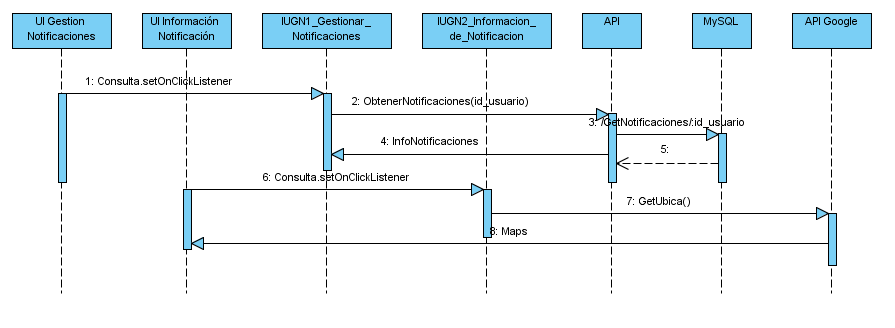
\includegraphics[width=1.0\textwidth]{AvancesPruebas/imagenes/GestionNotifica}}
	\caption{Diagrama secuencia de Notificaciones}
	\label{fig:Notificaciones}
\end{figure}
\begin{itemize}
	\item \textbf{Login.setOnClickListener:} 
\end{itemize}

La información que será enviada en caso de una notificación manual se describe a continuación:

\subsubsection{Información enviada en notificaciones manuales}

Para que un contacto registrado por el usuario pueda recibir una notificación, debe tener previamente los permisos para recibir información por parte del usuario, esto con la finalidad de proteger datos que el considere. Los datos que se envían se dividen en 4 tipos, los cuales se describen a continuación:

\begin{itemize}
	\item \textbf{Información Dispositivo}
	\begin{itemize}
		\item \textbf{Latitud}: Es la latitud que tiene el dispositivo en el momento que se manda la notificación.
		\item \textbf{Longitud}: Es la longitud que tiene el dispositivo en el momento que se manda la notificación.
	\end{itemize}

	\item \textbf{Información Médica}
	
	\begin{itemize}
		\item \textbf{Tipo de Sangre}: Es el tipo de sangre del usuario.
		\item \textbf{Enfermedad}: Enfermedad que tiene registrada el usuario.
		\item \textbf{No.Seguridad}: Es el número de seguridad social que registro el usuario.
	\end{itemize}

	\item \textbf{Información Personal}
	
	 \begin{itemize}
	 	\item \textbf{Nombre}: Es el nombre del usuario.
	 	\item \textbf{Primer Apellido}: Es el primer apellido del usuario.
	 	\item \textbf{Segundo Apellido}: Es el segundo apellido del usuario.
	 	\item \textbf{Fecha de nacimiento}: Es la fecha de nacimiento del usuario.
	 	\item \textbf{Sexo}: Es el sexo del usuario.
	 \end{itemize}
 
 	\item \textbf{Información Vehículo}
 	
 	\begin{itemize}
 		\item \textbf{Placas}: Es el número de placas del vehículo del usuario.
 		\item \textbf{Póliza}: Es el número de póliza del vehículo.
 		\item \textbf{Codigo OBD2}: Es el código recibido por el lector OBD2 y este es interpretado.
 	\end{itemize}
	
\end{itemize}

\subsection{Notificaciones Automáticas}

La figura \ref{fig:NotificaAuto} se muestra el diagrama de secuencia correspondiente al envió de notificaciones automáticas, es aquí donde se han establecido las reglas para el envió de alertas, mismas que se describen a continuación. Para el envío de notificaciones automáticas se tomaron en cuenta los siguientes aspectos:

\subsubsection{Información del dispositivo}

La información del dispositivo smartphone que se utilizó para la interpretación de un posible coche automovilístico es la siguiente:
\begin{itemize}
	\item \textbf{Ubicación}. Para hacer uso de la ubicación de un smartphone se realizó una conexión con el API de Google Maps, que con ayuda de sus métodos podemos obtener la latitud y longitud donde se encuentra, esto utilizando el A-GPS del smartphone.
	
	\item \textbf{Velocidad}. Para obtener la velocidad a la que se mueve el dispositivo que se encuentra en un vechículo en movimiento o en cualquier otro transporte que haya desplazamiento se tomaron en cuenta los siguientes aspectos:
	
	\begin{itemize}
		\item \textbf{Ubicación 1}. Es la ubicación inicial en la que se encuentra el dispositivo, esta ubicación está dada por longitud y latitud, misma que nos proporciona la API de Google.
		\item \textbf{Tiempo}. Es el tiempo que se tiene de referencia para obtener una nueva ubicación en el dispositivo.Para este caso se tomó la referencia de 2000 ms.
		\item \textbf{Ubicación 2}. Es la ubicación en la que se encuentra el dispositivo después de haber pasado el periodo de tiempo establecido.
		\item \textbf{Distancia}. Es la distancia que existe entre la ubicación 1 y la ubicación 2.
		\item \textbf{Velocidad}. Esta se determina con la distancia que existe entre la Ubicación 1 y Ubicación 2 así mismo con el tiempo que se tardo en actualizar el segundo punto. Para este cálculo se utilizo la formula $V = Distancia/Tiempo$, dando por hecho que se tuvo una aceleración uniforme, la cual es muy aproximada debido al tiempo en que se obtuvo una segunda ubicación.
	\end{itemize}

	\item \textbf{Cambios Giroscopio}. Se utilizaron los cambios bruscos en la posición del dispositivo, esta información la brinda el giroscopio del smartphone. 
	\item \textbf{Cambios Acelerómetro}. Se utilizó la información de los cambios bruscos de información en el acelerómetro.
	\item \textbf{Información ODB2}. Para poder saber el posible estado del vehículo, la aplicación espera obtener uno de los códigos establecidos como sensibles a la hora de un choque esto mediante.
\end{itemize}

Las siguientes gráficas muestran el comportamiento considerado como normal vs el comportamiento anormal en un choque automovilístico en un lapso de 100000 ms y el evento anormal en el lapso de 28000 ms - 38000 ms.

La figura \ref{fig:NotificaAutoV} muestra como se comportaría la velocidad de un coche en situaciones consideradas normales vs situaciones anormales (choque automovilístico).
\begin{figure}[htbp!]
	\centering
	\fbox{\includegraphics[width=1.0\textwidth]{AvancesPruebas/imagenes/VElocidadVS}}
	\caption{Gráfica Velocidad normal vs Velocidad anormal}
	\label{fig:NotificaAutoV}
\end{figure}
La figura \ref{fig:NotificaAutoG} muestra como se comportaría el giroscopio del dispositivo en una situación considerada normal  y en la figura \ref{fig:NotificaAutoGA} situaciones anormales (choque automovilístico), esto mientras se encuentra en un lugar fijo dentro del vehículo.
\begin{figure}[htbp!]
	\centering
	\fbox{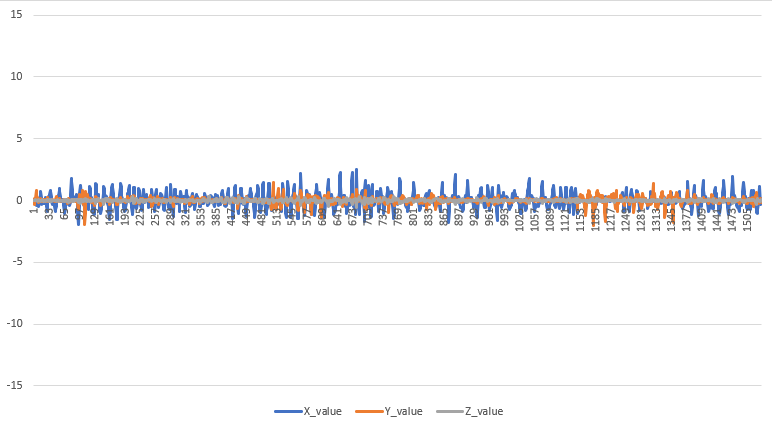
\includegraphics[width=1.0\textwidth]{AvancesPruebas/imagenes/GiroscopioN}}
	\caption{Gráfica Giroscopio anormal}
	\label{fig:NotificaAutoG}
\end{figure}
\begin{figure}[htbp!]
	\centering
	\fbox{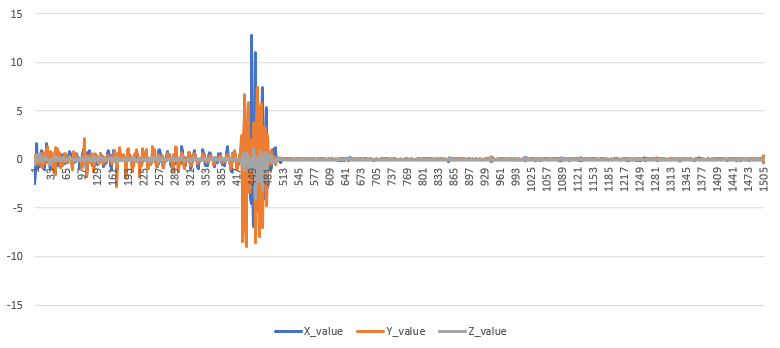
\includegraphics[width=1.0\textwidth]{AvancesPruebas/imagenes/GiroscopioA}}
	\caption{Gráfica Giroscopio normal}
	\label{fig:NotificaAutoGA}
\end{figure}

La figura \ref{fig:NotificaAutoA} muestra como se comportaría el Acelerómetro del dispositivo en una situación considerada normal, en la figura \ref{fig:NotificaAutoAA} situaciones anormales (choque automovilístico), esto mientras se encuentra en un lugar fijo dentro del vehículo.
\begin{figure}[htbp!]
	\centering
	\fbox{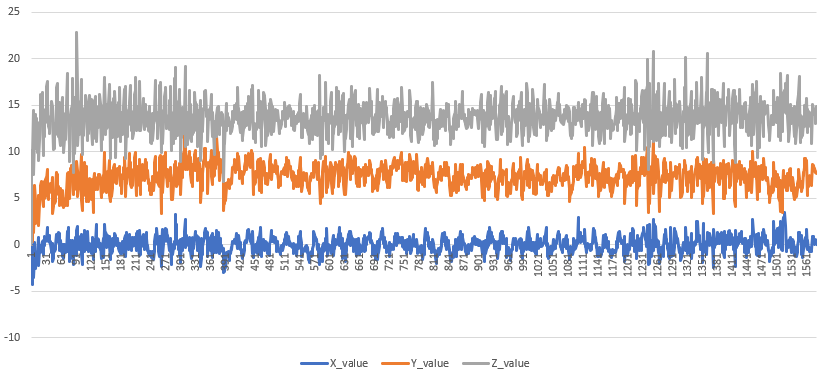
\includegraphics[width=1.0\textwidth]{AvancesPruebas/imagenes/AcelerometroN}}
	\caption{Gráfica Acelerómetro normal}
	\label{fig:NotificaAutoA}
\end{figure}

\begin{figure}[htbp!]
	\centering
	\fbox{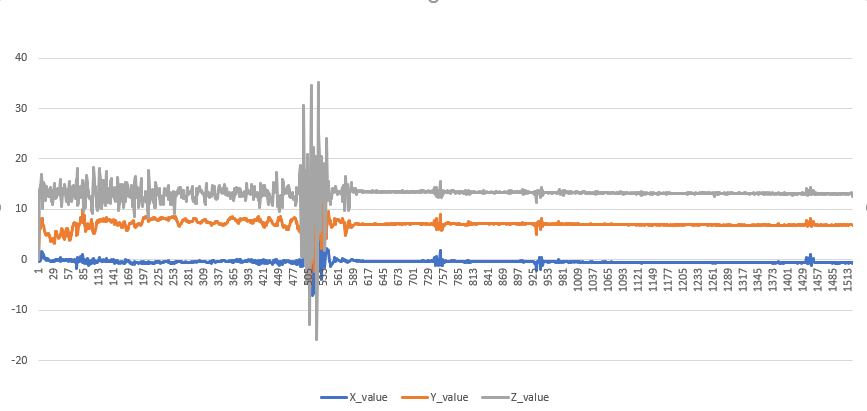
\includegraphics[width=1.0\textwidth]{AvancesPruebas/imagenes/AcelerometroA}}
	\caption{Gráfica Acelerómetro anormal}
	\label{fig:NotificaAutoAA}
\end{figure}

La figura \ref{fig:NotificaAutoO} muestra como se comportaría el obd2 que se encuentra conectado en el vehículo, esto en una situación considerada normal vs situaciones anormales (choque automovilístico). 
\begin{figure}[htbp!]
	\centering
	\fbox{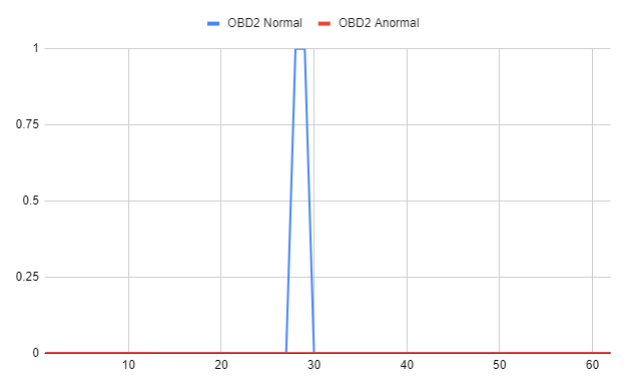
\includegraphics[width=1.0\textwidth]{AvancesPruebas/imagenes/OBD2vs}}
	\caption{Gráfica OBD2 normal vs OBD2 anormal}
	\label{fig:NotificaAutoO}
\end{figure}


\begin{figure}[htbp!]
	\centering
	\fbox{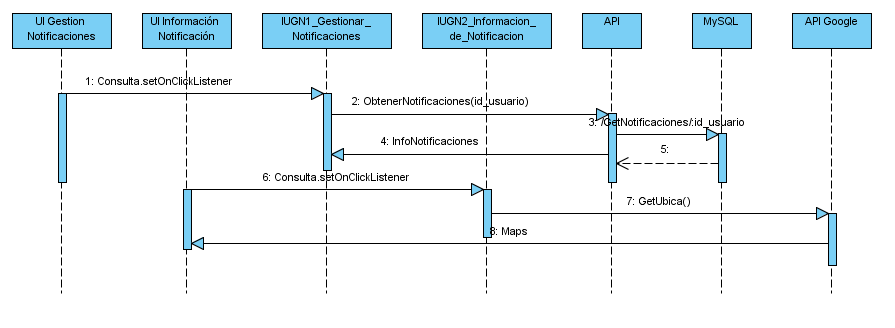
\includegraphics[width=1.0\textwidth]{AvancesPruebas/imagenes/GestionNotifica}}
	\caption{Diagrama secuencia Notificaciones Automáticas}
	\label{fig:NotificaAuto}
\end{figure}
\begin{itemize}
	\item \textbf{Login.setOnClickListener:} Es la acción que dispara el usuario, no recibe datos como parámetros, es el disparador.
\end{itemize}

\subsubsection{Información enviada en notificaciones automáticas}

Para que un contacto registrado por el usuario pueda recibir una notificación automática, debe tener previamente los permisos para recibir información por parte del usuario, esto con la finalidad de proteger datos que el considere. Los datos que se envían se dividen en 4 tipos, los cuales se describen a continuación:

\begin{itemize}
	\item \textbf{Información Dispositivo}
	\begin{itemize}
		\item \textbf{Latitud}: Es la latitud que tiene el dispositivo en el momento que se manda la notificación.
		\item \textbf{Longitud}: Es la longitud que tiene el dispositivo en el momento que se manda la notificación.
	\end{itemize}
	
	\item \textbf{Información Médica}
	
	\begin{itemize}
		\item \textbf{Tipo de Sangre}: Es el tipo de sangre del usuario.
		\item \textbf{Enfermedad}: Enfermedad que tiene registrada el usuario.
		\item \textbf{No.Seguridad}: Es el número de seguridad social que registro el usuario.
	\end{itemize}
	
	\item \textbf{Información Personal}
	
	\begin{itemize}
		\item \textbf{Nombre}: Es el nombre del usuario.
		\item \textbf{Primer Apellido}: Es el primer apellido del usuario.
		\item \textbf{Segundo Apellido}: Es el segundo apellido del usuario.
		\item \textbf{Fecha de nacimiento}: Es la fecha de nacimiento del usuario.
		\item \textbf{Sexo}: Es el sexo del usuario.
	\end{itemize}
	
	\item \textbf{Información Vehículo}
	
	\begin{itemize}
		\item \textbf{Placas}: Es el número de placas del vehículo del usuario.
		\item \textbf{Póliza}: Es el número de póliza del vehículo.
		\item \textbf{Codigo OBD2}: Es el código recibido por el lector OBD2 y este es interpretado.
	\end{itemize}
	
\end{itemize}

\subsubsection{Diagrama flujo Notificaciones Automáticas}

En la figura \ref{fig:DiagramaNA} se aprecia como es que se evalúan y generan las notificaciones automáticas, esto en caso que se haya interpretado un posible coche automovilístico.


\begin{figure}[htbp!]
	\centering
	\fbox{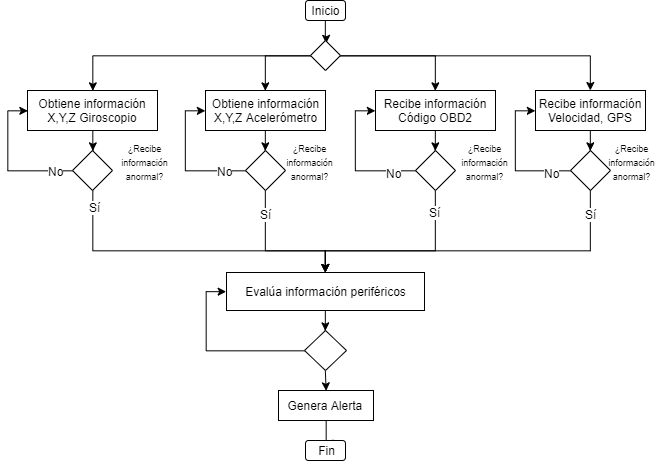
\includegraphics[width=1.0\textwidth]{AvancesPruebas/imagenes/DiagramaAletrta}}
	\caption{Diagrama flujo Notificaciones Automáticas}
	\label{fig:DiagramaNA}
\end{figure}

\subsubsection{Eventos de Notificaciones Automáticas}

Con ayudas de las gráficas obtenidas en la sección \textbf{Información del dispositivo}, se determinó la siguiente tabla, la cual muestra cuando se podrá ser disparada una notificación automática.

\begin{figure}[htbp!]
	\centering
	\fbox{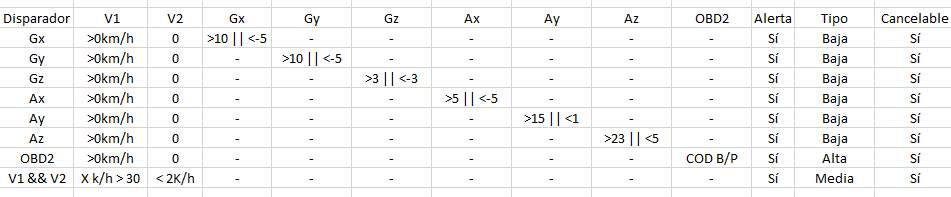
\includegraphics[width=1.0\textwidth]{AvancesPruebas/imagenes/Disparadores}}
	\caption{Disparadores Notificación Automática}
	\label{fig:Disparadores}
\end{figure}

En un inicio se tomará la gravedad que se muestra en la figura \ref{fig:Disparadores}, esta podrá cambiar dependiendo de los eventos que se presenten en el dispositivo móvil, vehículo. La definición de como es que cambiarán los eventos, se establece en la figura \ref{fig:Combinaciones}.


\begin{figure}[htbp!]
	\centering
	\fbox{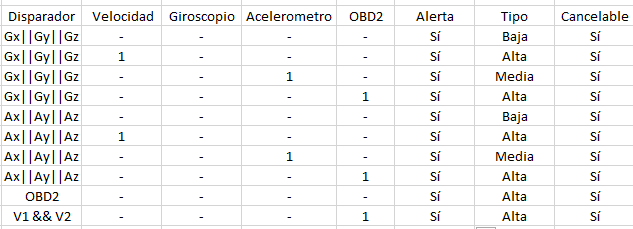
\includegraphics[width=1.0\textwidth]{AvancesPruebas/imagenes/Combinaciones}}
	\caption{Combinaciones Notificaciones Automáticas}
	\label{fig:Combinaciones}
\end{figure}



 